% =====================================================================
%  kubemend --- technical report
%  Compiles with pdfLaTeX on Overleaf. Single file, no external assets
%  required except docs/console.jpg (optional; guarded below).
% =====================================================================
\documentclass[11pt,a4paper]{article}

\usepackage[T1]{fontenc}
\usepackage[utf8]{inputenc}
\usepackage{mathptmx}                 % Times text and math
\usepackage[scaled=0.85]{helvet}      % sans for headings
\usepackage{courier}
\usepackage{amssymb}
\usepackage{microtype}
\usepackage[margin=1in]{geometry}
\usepackage{booktabs}
\usepackage{tabularx}
\usepackage{xcolor}
\usepackage{listings}
\usepackage{newunicodechar}
\usepackage{enumitem}
\usepackage{caption}
\usepackage{graphicx}
\usepackage{tikz}
\usetikzlibrary{arrows.meta,positioning,fit,backgrounds}
\usepackage[colorlinks=true,linkcolor=linknavy,citecolor=linknavy,
            urlcolor=linknavy]{hyperref}

% ---------------------------------------------------------------- colours
\definecolor{linknavy}{HTML}{1D4ED8}
\definecolor{rulegrey}{HTML}{6B7280}
\definecolor{codebg}{HTML}{F7F7F5}
\definecolor{codeline}{HTML}{E4E4E1}
\definecolor{okgreen}{HTML}{15803D}
\definecolor{badred}{HTML}{B91C1C}
\definecolor{warnamber}{HTML}{A16207}

% ---------------------------------------------------------------- listings
\lstdefinestyle{shell}{
  basicstyle=\ttfamily\footnotesize,
  backgroundcolor=\color{codebg},
  frame=single,
  rulecolor=\color{codeline},
  framesep=6pt,
  xleftmargin=10pt,
  xrightmargin=4pt,
  breaklines=true,
  breakatwhitespace=true,
  columns=fullflexible,
  keepspaces=true,
  showstringspaces=false,
  extendedchars=true,
}
\lstdefinestyle{pycode}{
  style=shell,
  language=Python,
  keywordstyle=\color{linknavy},
  commentstyle=\color{rulegrey}\itshape,
  stringstyle=\color{okgreen},
}
\lstset{style=shell}

% The demo transcripts are reproduced verbatim, and contain glyphs the Times
% typewriter font has no slot for. newunicodechar maps them to maths
% equivalents, which works inside listings where lstlisting's own `literate`
% does not for multi-byte characters under pdfLaTeX.
\newunicodechar{✓}{\textcolor{okgreen}{\ensuremath{\checkmark}}}
\newunicodechar{✗}{\textcolor{badred}{\ensuremath{\times}}}
\newunicodechar{→}{\ensuremath{\rightarrow}}
\newunicodechar{↳}{\ensuremath{\hookrightarrow}}
\newunicodechar{·}{\ensuremath{\cdot}}

% ---------------------------------------------------------------- headings
\usepackage{titlesec}
\titleformat{\section}{\sffamily\large\bfseries}{\thesection}{0.7em}{}
\titleformat{\subsection}{\sffamily\normalsize\bfseries}{\thesubsection}{0.7em}{}
\titleformat{\subsubsection}{\sffamily\small\bfseries}{\thesubsubsection}{0.7em}{}
\setlist[itemize]{leftmargin=1.3em,itemsep=2pt,topsep=3pt}
\setlist[enumerate]{leftmargin=1.6em,itemsep=2pt,topsep=3pt}
\captionsetup{font=small,labelfont={sf,bf}}

% ---------------------------------------------------------------- macros
\newcommand{\code}[1]{\texttt{\small #1}}
\newcommand{\kubemend}{\textsc{kubemend}}

% =====================================================================
\begin{document}

\begin{titlepage}
\centering
\vspace*{2.2cm}

{\sffamily\Huge\bfseries kubemend\par}
\vspace{0.7cm}
{\sffamily\Large A Kubernetes remediation agent whose only\\[2pt]
write surface is a git commit\par}

\vspace{1.6cm}
{\large Srivatsa Kamballa\par}
\vspace{0.3cm}
{\small \href{https://github.com/Srivatsa03/kubemend}{github.com/Srivatsa03/kubemend}\par}
\vspace{0.2cm}
{\small Version 0.1.0 (alpha) \quad\textbullet\quad Apache-2.0 \quad\textbullet\quad August 2026\par}

\vspace{1.8cm}
\begin{minipage}{0.86\textwidth}
\small
\noindent\textbf{Abstract.}
Autonomous remediation for Kubernetes is limited less by diagnostic quality than
by trust. A tool that can identify a crash loop is straightforward to build; a
tool an operator will permit to act on production unattended is not, and the
obstacle is that no convincing answer exists to the question of what prevents it
doing something catastrophic without supervision. \kubemend{} is an attempt at
that answer, constructed so that the safety properties are structural rather
than behavioural. The agent holds no cluster credentials and issues no write to
the Kubernetes API. It reads cluster state with read-only verbs, selects from a
closed set of six typed actions each carrying the state it found and the state
it intends, subjects the resulting plan to a pure-function policy gate, and
emits the change as a commit to a GitOps repository, which an existing
reconciler carries to the cluster. Undoing the agent is \code{git revert}.
After committing, it verifies: it polls the workload, requires two consecutive
clean observations before declaring recovery, and withdraws its own commit when
presented with positive evidence that the fix did not hold. Every run is
recorded to an append-only incident log, which yields the measurement the field
generally omits --- the agent's revert rate, its own accuracy on real outcomes.
On a live k3d cluster the system demonstrates both terminal outcomes in a single
run: one fix recovered in 26 seconds and was kept, and a second, applied against
two consecutive bad releases, was still failing after 76 seconds and was
reverted automatically. The implementation is 3{,}248 lines of Python with no
runtime dependencies, covered by 157 tests, with continuous integration
exercising the full loop against a real cluster on every push.
\end{minipage}

\vfill
{\footnotesize The planner is deterministic. There is no language model in the decision path;
see \S\ref{sec:limits}.\par}
\end{titlepage}

\tableofcontents
\newpage

% =====================================================================
\section{The problem is trust, not detection}

Every observability vendor can tell an operator that a pod is in
\code{CrashLoopBackOff}. Very few of their agents are permitted to do anything
about it, and the reason is not model quality. It is that granting write access
to a production cluster requires an answer to a specific question --- what stops
this from doing something catastrophic at three in the morning --- and
``the model is usually careful'' is not an answer. It is a statement about
average behaviour offered in response to a question about worst-case behaviour.

The gap has a structural cause. An agent that emits shell commands, \code{kubectl}
invocations, or freely-generated manifests has an unbounded action space. Three
consequences follow immediately, and none of them are implementation defects
that a better model would resolve:

\begin{itemize}
  \item The set of things it might do cannot be enumerated, so it cannot be reviewed in advance.
  \item The blast radius of a proposed change cannot be computed before it runs.
  \item There is no mechanical inverse, so recovery from a bad action is itself an act of judgement under pressure.
\end{itemize}

Every safety property an operator would want is therefore unavailable
\emph{in principle}, not merely unimplemented. \kubemend{} starts from the
opposite constraint: restrict the action space until those properties become
computable, then let the agent diagnose as freely as it likes inside it. The
design separates the two concerns deliberately --- \textbf{diagnose broadly, act
narrowly} --- and every constraint on the acting half is code with tests rather
than an instruction in a prompt.

\subsection{The central design decision}

\kubemend{} has no cluster credentials capable of mutation and issues no write to
the Kubernetes API. Its only write surface is a commit to the GitOps repository
that already defines the cluster. An existing reconciler --- Argo~CD, Flux, or
whatever the team already runs --- carries the change the rest of the way.

This single choice inherits an entire safety apparatus rather than
reimplementing it:

\begin{itemize}
  \item \textbf{An audit trail} exists because git is one, with authorship, timestamps and message.
  \item \textbf{Review before rollout} is available because a pull request is the native unit of review.
  \item \textbf{Rollback} is \code{git revert}, a command every operator on the team already knows at 3am.
  \item \textbf{Reconciliation} is someone else's well-tested problem.
\end{itemize}

It also imposes a real constraint, which is the point: an action that cannot be
expressed as an edit to a manifest cannot be performed at all. A rolling restart
has no manifest representation, so \kubemend{} refuses it with a reason rather
than approximating it with an annotation nobody asked for.

% =====================================================================
\section{Architecture}

The loop is six stages, each a pure function of the previous stage's output
wherever it can be. Purity is not stylistic here: it is what allows the entire
decision path to be tested against recorded cluster state, with no cluster
present and no mocking of the parts that matter.


\begin{enumerate}
  \item \textbf{Read.} Cluster state via read-only verbs on the existing kubeconfig, or a recorded JSON snapshot.
  \item \textbf{Detect.} Eight rules produce typed \code{Finding} objects with severity and evidence.
  \item \textbf{Plan.} Findings are grouped per workload; each incident yields at most one plan.
  \item \textbf{Gate.} A pure function returns a verdict: refused, or permitted at a specific autonomy level.
  \item \textbf{Emit.} The plan is rendered as a surgical manifest edit and committed, or opened as a pull request.
  \item \textbf{Verify.} The workload is polled; a fix that does not hold is withdrawn by \code{git revert}.
\end{enumerate}

\begin{figure}[h]
\centering
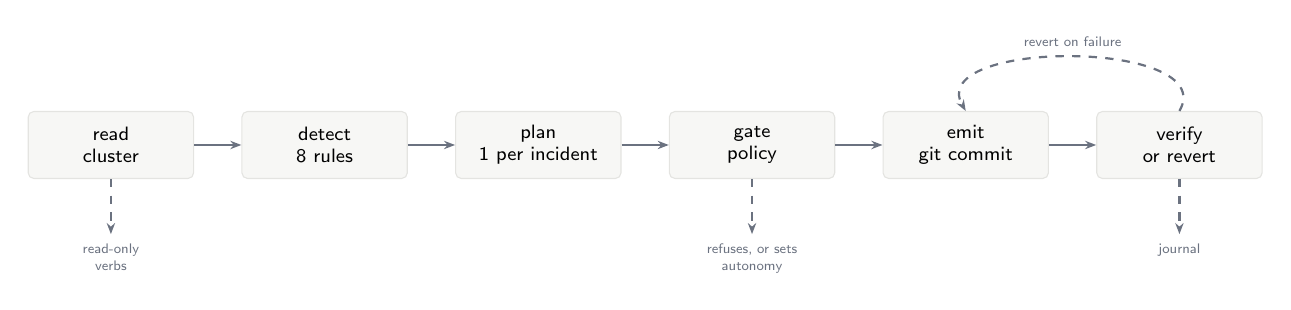
\begin{tikzpicture}[
  node distance=6mm,
  box/.style={draw=codeline,fill=codebg,rounded corners=2pt,
              minimum height=8.5mm,minimum width=21mm,align=center,
              font=\sffamily\scriptsize,inner sep=3pt},
  arrow/.style={-{Stealth[length=4pt]},draw=rulegrey,thick},
]
\node[box] (read)   {read\\\scriptsize cluster};
\node[box,right=of read]   (detect) {detect\\\scriptsize 8 rules};
\node[box,right=of detect] (plan)   {plan\\\scriptsize 1 per incident};
\node[box,right=of plan]   (gate)   {gate\\\scriptsize policy};
\node[box,right=of gate]   (emit)   {emit\\\scriptsize git commit};
\node[box,right=of emit]   (verify) {verify\\\scriptsize or revert};

\draw[arrow] (read) -- (detect);
\draw[arrow] (detect) -- (plan);
\draw[arrow] (plan) -- (gate);
\draw[arrow] (gate) -- (emit);
\draw[arrow] (emit) -- (verify);

\node[below=7mm of read,font=\sffamily\tiny,text=rulegrey,align=center]
  (l1) {read-only\\verbs};
\node[below=7mm of gate,font=\sffamily\tiny,text=rulegrey,align=center]
  (l2) {refuses, or sets\\autonomy};
\node[below=7mm of verify,font=\sffamily\tiny,text=rulegrey,align=center]
  (l3) {journal};

\draw[arrow,dashed] (read) -- (l1);
\draw[arrow,dashed] (gate) -- (l2);
\draw[arrow,dashed] (verify) -- (l3);

\draw[arrow,dashed] (verify.north) to[out=60,in=120] node[above,font=\sffamily\tiny,text=rulegrey]{revert on failure} (emit.north);
\end{tikzpicture}
\caption{The remediation loop. Everything left of \emph{emit} is a pure function
of recorded cluster state and therefore testable without a cluster.}
\end{figure}

Every stage writes to an append-only incident log (\S\ref{sec:journal}), which
is what makes the agent's own accuracy measurable rather than asserted.

% =====================================================================
\section{Detection}

Detection is deliberately the least constrained part of the system, because
being wrong here costs a false report rather than a bad change. Eight rules run
over cluster JSON and emit findings carrying rule, severity, target and
structured evidence.

\begin{table}[h]
\centering
\small
\begin{tabularx}{\textwidth}{@{}l l X@{}}
\toprule
\textbf{Rule} & \textbf{Severity} & \textbf{What it catches} \\
\midrule
\code{crashloop}         & critical & Container the kubelet has given up restarting promptly \\
\code{oomkilled}         & critical & Killed by the kernel for exceeding its memory limit \\
\code{image\_pull}       & critical & Bad tag, bad registry, or missing pull credentials \\
\code{config\_error}     & critical & References a ConfigMap or Secret that does not exist \\
\code{rollout\_stuck}    & critical & Rollout past its progress deadline \\
\code{replica\_shortfall}& critical / warning & Fewer replicas available than desired \\
\code{unschedulable}     & warning  & No node can fit the pod \\
\code{flapping}          & warning  & Restarting repeatedly while still reporting healthy \\
\bottomrule
\end{tabularx}
\caption{The detection rules. Severity describes how bad the observed condition
is, independent of confidence in any fix.}
\end{table}

\code{flapping} is the rule worth singling out. The pod is up, dashboards are
green, nothing pages, and the container has died eleven times today. That is the
failure mode most likely to survive unnoticed for weeks, and it is invisible to
any check that asks only whether pods are running.

% =====================================================================
\section{Typed actions}

\kubemend{} never emits commands. It selects from a closed set of six typed
actions, and every action carries both the state it found (\code{before}) and
the state it intends (\code{after}).

\begin{table}[h]
\centering
\small
\begin{tabularx}{\textwidth}{@{}l X l@{}}
\toprule
\textbf{Action} & \textbf{Effect} & \textbf{Manifest field} \\
\midrule
\code{scale}          & Change replica count                    & \code{spec.replicas} \\
\code{rollback}       & Revert a workload to a prior revision   & restored from git history \\
\code{restart}        & Trigger a rolling restart               & none --- refused on emission \\
\code{set\_resources} & Adjust requests or limits               & \code{...containers.\emph{c}.resources} \\
\code{set\_image}     & Pin or correct a container image        & \code{...containers.\emph{c}.image} \\
\code{set\_probe}     & Adjust probe timings or thresholds      & none --- refused on emission \\
\bottomrule
\end{tabularx}
\caption{The closed action set. Each entry is a change an experienced operator
makes routinely, whose effect is local and whose reversal is mechanical.}
\end{table}

Three properties follow directly from the type, not from the agent's care:

\begin{itemize}
  \item \textbf{Reversible by construction.} An action holds \code{before} and \code{after}, so its inverse is a field swap. An action whose \code{before} could not be captured is refused up front, rather than discovered to be irreversible at rollback time.
  \item \textbf{Blast radius computable before execution.} Every action declares the pods it disrupts, so a plan is measured and refused while it is still text.
  \item \textbf{Reviewable.} A typed action renders to a deterministic diff. A reviewer sees a bounded change, not a prompt's output.
\end{itemize}

Adding a kind to this set is a security decision rather than a feature decision,
because it widens what an autonomous process may do to a live cluster.

\subsection{One plan per incident, and the freedom to abstain}

An incident is something that happened to a service, and responders handle them
one at a time. Batching unrelated problems into a single change would trip every
blast-radius limit simultaneously and couple the fate of unrelated services.
Separate plans are separately reviewable, appliable and revertible.

Abstention is treated as a correct outcome rather than a failure to be minimised.
On the shipped fixture --- a recorded snapshot of a cluster having a bad
afternoon --- \textbf{13 findings produce 4 plans, and 5 findings produce no
action at all.} A missing ConfigMap needs a value the agent has no business
inventing. An unschedulable pod is a capacity decision. A container restarting
for unclear reasons needs a human to read the logs. Reporting these clearly and
stopping is the correct behaviour, and the test suite asserts it.

% =====================================================================
\section{The policy gate}

The gate is a pure function from (plan, policy) to verdict, with no model in the
loop. It enforces six properties.

\begin{enumerate}
  \item \textbf{Protected namespaces are excluded outright.} \code{kube-system}, \code{argocd}, \code{flux-system} and similar are refused rather than guarded by a threshold. Touching them can remove the machinery that would let you recover.
  \item \textbf{Only action kinds named in policy}, with everything else denied by default.
  \item \textbf{Blast radius bounded} on pods, workloads and namespaces --- for the plan as a whole, since three individually harmless restarts are not a harmless change.
  \item \textbf{No action without a computable undo.}
  \item \textbf{Flap protection.} A cluster that has already needed several fixes this window is a human's problem, not a loop's.
  \item \textbf{An unconfigured \code{Policy()} permits nothing.} A permissive default is the difference between a bounded assistant and an unsupervised process with cluster credentials.
\end{enumerate}

Policy is data, not code, so the rules governing an autonomous system are
themselves reviewable, diffable and revertible --- the same property the agent's
own actions are required to have.

\subsection{Three levels of autonomy, granted per action}

Trust is granted per action class and per environment rather than assumed
globally, mirroring the crawl, walk, run progression that operations teams
already use.

\begin{table}[h]
\centering
\small
\begin{tabularx}{\textwidth}{@{}l X@{}}
\toprule
\textbf{Level} & \textbf{What happens} \\
\midrule
\code{report}  & Findings only. Nothing is proposed. \\
\code{propose} & A branch and a pull request, for human review. \\
\code{apply}   & Committed to the GitOps branch unattended. \\
\bottomrule
\end{tabularx}
\end{table}

Under the shipped conservative policy only \code{rollback} may apply unattended,
because it moves a workload to a state that demonstrably ran in this cluster and
its inverse is exact. Everything else waits for a human.

\textbf{A plan's autonomy is the minimum across its actions.} One action
requiring review holds back the whole plan, because applying the safe half of a
plan that was reasoned about as a unit is frequently worse than applying none of
it.

\begin{table}[h]
\centering
\small
\begin{tabularx}{\textwidth}{@{}l l l X@{}}
\toprule
\textbf{Workload} & \textbf{Action} & \textbf{Verdict} & \textbf{Reason} \\
\midrule
\code{payments/checkout}    & \code{rollback}       & \textcolor{okgreen}{apply}   & within all limits \\
\code{jobs/report-worker}   & \code{rollback}       & \textcolor{okgreen}{apply}   & within all limits \\
\code{payments/api}         & \code{set\_resources} & \textcolor{warnamber}{propose} & \code{autonomy\_ceiling} \\
\code{kube-system/coredns}  & \code{rollback}       & \textcolor{badred}{refused}  & \code{protected\_namespace} \\
\bottomrule
\end{tabularx}
\caption{Gate verdicts on the shipped fixture under the conservative policy.
The identical \code{rollback} action is applied on one workload and refused on
another purely on namespace, which is the gate doing its job.}
\end{table}

% =====================================================================
\section{Writing the fix}

\subsection{Rollback is a git operation, not a computed edit}

In a GitOps repository the manifest is the source of truth, so returning a
workload to its previous revision means restoring the file to its previous
committed state. Nothing is reconstructed --- the prior version is present in the
history, byte for byte, comments and all. This falls out of the architecture
rather than being engineered, and it is the strongest single argument for routing
an agent's actions through git.

\subsection{The diff is one line}

The obvious way to edit a manifest is to parse the YAML, mutate the object, and
serialise it back. That produces a correct file and a useless commit: the
serialiser rewrites the whole document, drops comments, reorders keys and
normalises quoting, so a reviewer sees three hundred changed lines when the
change was one number.

The entire value of routing actions through git is that a human can read the diff
before it reaches the cluster. A commit that reformats the file is unreviewable,
which defeats the purpose. \kubemend{} therefore performs \emph{surgical} text
edits against an indentation-path tracker rather than parsing and dumping.
Trailing comments survive, including the exact whitespace preceding them.

\begin{lstlisting}[caption={An emitted change. One line, comment and spacing intact.}]
-          image: nginx:1.27-alpine-typo   # known good
+          image: nginx:1.27-alpine   # known good
\end{lstlisting}

\subsection{It refuses more than it writes}

\begin{itemize}
  \item \textbf{A workload with no manifest} is reported, never created.
  \item \textbf{A value that drifted} --- the repository says something other than what the cluster reported --- is left alone. Somebody changed it, and their change is not the agent's to discard.
  \item \textbf{A field that does not exist} is not added. Inventing a resource limit the author never wrote is a different class of change from adjusting one that is there.
  \item \textbf{An action with no manifest representation}, such as a rolling restart, is refused with a reason rather than approximated.
  \item \textbf{A dirty working tree} blocks emission entirely, so an agent's commit never absorbs somebody's in-progress edit.
\end{itemize}

\subsection{The commit message is the evidence}

Every commit carries what produced it, and closes with the instruction that
matters.

\begin{lstlisting}[caption={A generated commit message, verbatim from the live demo.}]
rollback payments/deployment/checkout

Observed:
  [critical] cannot pull image nginx:1.27-alpine-typo for checkout-6d78fb9788-t488h

Changed:
  restored clusters/prod/checkout.yaml to f14c37f1
    reason: image_pull: cannot pull image nginx:1.27-alpine-typo

Blast radius: 2 pod(s) across 1 workload(s).
Undo: git revert this commit.
\end{lstlisting}

Plans held at \code{propose} push their branch and open a pull request whose body
is this message. A repository with no remote, or a missing \code{gh}, is reported
rather than treated as an error, since that is the normal case for a local
checkout.

% =====================================================================
\section{Verification, and the discipline of undoing}

A remediation loop that stops at ``committed'' is half a loop. The agent has
acted on a diagnosis that may have been wrong, and until something checks, the
cluster is in a state nobody has confirmed is better than the one it replaced.

Recovery is defined narrowly: \textbf{the findings that motivated the change are
gone, and no new critical finding has appeared on that workload.} Not ``the
workload is perfect'' --- a service can carry a warning for weeks --- and not
``the pods are running'', which is true moments before a crash loop starts.

A workload must read clean \textbf{twice consecutively}, because a rollout looks
briefly healthy as it begins. A \code{settle} grace period precedes the first
check, since a reconciler needs a moment to apply the commit and checking
immediately would reliably observe the old state and call it a failure.

\begin{table}[h]
\centering
\small
\begin{tabularx}{\textwidth}{@{}l X l@{}}
\toprule
\textbf{Outcome} & \textbf{Meaning} & \textbf{Reverts?} \\
\midrule
\code{recovered}     & the motivating findings are gone                & no \\
\code{still\_failing}& they remain, or a new critical one appeared     & \textbf{yes} \\
\code{indeterminate} & the cluster could not be read                   & no \\
\bottomrule
\end{tabularx}
\end{table}

The third row is the one worth arguing about, and it encodes two decisions that
matter more than the polling mechanics.

\textbf{Silence is not success.} A poll that cannot reach the cluster proves
nothing, so it never counts toward recovery --- and, more subtly, it \emph{breaks
the recovery streak} rather than being skipped. Two clean reads either side of a
blind one are not two consecutive observations, and allowing silence to bridge
them would contradict the rule the module is built on. This was originally
implemented the other way; a test asserted the correct behaviour and the
implementation was changed to match it, on the grounds that the module's own
stated contract was the authority.

\textbf{Indeterminate does not trigger a revert.} Reverting on positive evidence
of continued failure is right. Reverting because the API server was briefly
unreachable would undo a fix that may have worked, on no evidence at all, and
convert a network blip into a second production change. An unverifiable outcome
therefore stops and asks for a human.

When it does revert, it uses \code{git revert} rather than a reset. The history
of an automated system acting on production is worth keeping, and a reviewer
should see both that it acted and that it withdrew.

% =====================================================================
\section{The incident log}
\label{sec:journal}

A single run answers ``what is wrong now''. The questions that decide whether an
automated system deserves more autonomy are all longitudinal, and none of them
are answerable from standard output. Every run therefore records what it saw,
decided, wrote and confirmed to an append-only SQLite file at
\code{\~{}/.kubemend/journal.db}.

Two numbers come out of it that were previously unavailable.

\begin{quote}
\textbf{Revert rate} is the agent's own accuracy --- how often its fix failed to
hold and it withdrew its own commit. It is the only honest input to the question
``should this be allowed to \code{apply} rather than \code{propose}?'', and a
tool that quietly declined to measure it would be asking for trust it had not
earned.
\end{quote}

\begin{quote}
\textbf{Repeat offenders} are the workloads a rollback keeps papering over.
Something that crash-loops every week does not have a bad release, it has a bug,
and the log is what makes that visible instead of letting three successful
rollbacks look like three successes.
\end{quote}

Refusals are recorded alongside changes: what the gate declined to touch, and
why, is as much a part of the audit trail as what it wrote.

Two engineering choices are worth stating. Storage is standard-library
\code{sqlite3}, so the zero-dependency property holds and the log remains a
single file that can be copied, inspected with any tool, or deleted. And
\textbf{bookkeeping never breaks remediation}: every write is wrapped, an
unwritable journal degrades to a note in the output, and the run continues.
Failing to fix a broken cluster because a log file was read-only would be a poor
trade.

\begin{lstlisting}[caption={\code{kubemend log}, from the live demo run.}]
  incident log   /tmp/kubemend-demo-journal.db

  2026-08-15 16:46:25  reverted      payments/deployment/checkout
      cannot pull image nginx:1.27-broken-b for checkout-598f76497b-tmtwg
  2026-08-15 16:44:46  verified      payments/deployment/checkout
      cannot pull image nginx:1.27-alpine-typo for checkout-6d78fb9788-449mb

  totals   across 2 run(s)

    incidents   2
    committed   2
    refused     0
    verified    1
    revert rate 50%  (1 of 2 fixes did not hold)

  keeps coming back   a rollback is not going to fix these

      2x  payments/checkout
\end{lstlisting}

% =====================================================================
\section{The console}

\code{kubemend log} answers a question the operator already knew to ask. The
console serves the other mode: scanning a week of automated changes to production
and stopping at the one that looks wrong. Each incident opens to the full audit
trail --- the evidence observed, the action selected with \emph{both} its
\code{before} and \code{after}, the commit, the verification outcome, and the
revert if there was one.

\IfFileExists{console.jpg}{%
  \begin{figure}[h]\centering
  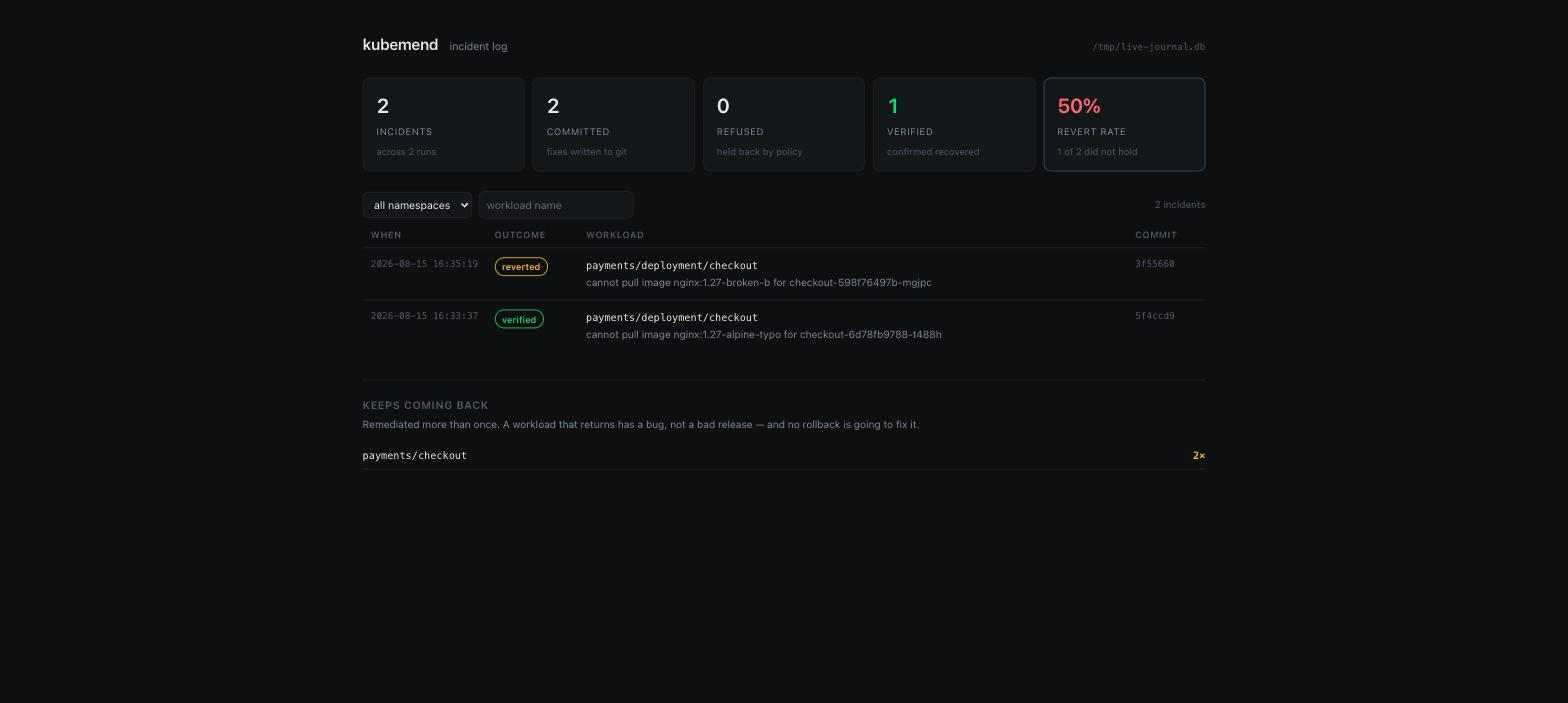
\includegraphics[width=\textwidth]{console.jpg}
  \caption{The console, showing real output from the live demo: two incidents on
  one workload, one fix that held and one that did not.}
  \end{figure}}{%
  \begin{center}\small\itshape
  (Screenshot \code{docs/console.jpg} not found in the Overleaf project;
  upload it alongside this file to include it.)\end{center}}

Three constraints shaped it, and each was a choice rather than an accident.

\begin{itemize}
  \item \textbf{Read-only, structurally rather than by policy.} There are no write routes at all, so nothing reachable from a browser can touch a cluster or a repository. The only write surface in this project is a git commit, and a console with a ``remediate now'' button would quietly make that claim untrue. \code{POST}, \code{PUT}, \code{DELETE} and \code{PATCH} are refused explicitly and covered by tests.
  \item \textbf{Localhost by default.} The journal is an inventory of what is fragile in a cluster --- workloads, images, namespaces, failure modes. A \code{--host} flag exists for people who mean it, and the server says so on startup.
  \item \textbf{Standard library only.} \code{http.server} over the same SQLite file. Installing a web framework in order to look at a local database would be a poor reason to break the dependency promise.
\end{itemize}

\subsection{An instructive bug}

The console initially shared one SQLite connection across the threaded server.
SQLite connections are bound to their creating thread, so every request after the
first failed --- and failed \emph{silently}, because the journal's read path
swallows errors by design so that bookkeeping cannot break remediation. The
symptom was an empty list rendered as ``no incidents'', which is a wrong answer
disguised as a valid one.

The fix is a connection per request, which is cheap for SQLite and has the
welcome side effect that a console reading a file a \code{remediate} run is still
appending to shows what was just written. The regression test drives a real
socket rather than calling the router in-process, because an in-process call
would have passed happily against the broken design; this was confirmed by
reproducing the failure before trusting the test.

% =====================================================================
\section{Evaluation}

\subsection{Offline, against a recorded cluster}

The repository ships a snapshot of a cluster with several simultaneous problems,
so the whole analysis path runs with nothing installed.

\begin{lstlisting}
$ kubemend diagnose --snapshot fixtures/broken-cluster.json

  kubemend   13 finding(s), 4 incident(s), policy 'conservative'
\end{lstlisting}

Thirteen findings become four plans; five findings produce no action at all. Of
the four plans, one is refused outright for touching a protected namespace, one
is held at \code{propose}, and two are permitted to \code{apply}.

\subsection{Live, on a real cluster}

\code{demo/run.sh} stands up a k3d cluster and a git repository holding its
manifests, applies the repository the way Argo~CD or Flux would, ships a release
that breaks, and lets \kubemend{} read the cluster and write the fix back. The
committed transcript in \code{demo/transcript.txt} is the verbatim output of a
real run.

The demo proves \emph{both} terminal outcomes, which matters more for an
unattended system than proving the happy path twice.

\paragraph{A fix that works.} A bad image tag is shipped. \kubemend{} detects the
pull failure, restores the manifest from git history, commits, and watches.

\begin{lstlisting}
      ✓ APPLY    payments/deployment/checkout
          restored clusters/prod/checkout.yaml to f14c37f1
          commit 9465b30a on main
          -          image: nginx:1.27-alpine-typo   # known good
          +          image: nginx:1.27-alpine   # known good
          watching for recovery...
          recovered after 26s
    1 commit(s) written.
\end{lstlisting}

\paragraph{A fix that does not.} The demo then ships \emph{two} bad releases in a
row, so that rolling back one still leaves the workload broken. \kubemend{}
commits its rollback, fails to observe recovery, and withdraws its own change.

\begin{lstlisting}
      ✓ APPLY    payments/deployment/checkout
          restored clusters/prod/checkout.yaml to 92a6903d
          commit 9b07e933 on main
          watching for recovery...
          still failing after 76s: cannot pull image nginx:1.27-broken-a
          reverted in 0b0d81f4
    0 commit(s) written.

   c2b3faa Revert "rollback payments/deployment/checkout"
   9b07e93 rollback payments/deployment/checkout
   9d637fb bad release B
\end{lstlisting}

The repository ends the run in the state a human last approved. The agent never
called the Kubernetes API to change anything: it read the cluster, committed a
fix, watched, kept the one that worked and reverted the one that did not.

\begin{table}[h]
\centering
\small
\begin{tabularx}{\textwidth}{@{}l l l X@{}}
\toprule
\textbf{Scenario} & \textbf{Outcome} & \textbf{Time to verdict} & \textbf{Action taken} \\
\midrule
One bad release  & \code{recovered}      & 26\,s & commit kept \\
Two bad releases & \code{still\_failing} & 76\,s & commit reverted automatically \\
\bottomrule
\end{tabularx}
\caption{Live k3d results, from the committed transcript. Wall-clock timings vary
between runs with cluster scheduling; the outcomes do not.}
\end{table}

Read separately these are two anecdotes. The incident log turns them into the
measurement the project is actually arguing about: \textbf{a 50\% revert rate,
computed from real outcomes rather than claimed}, together with
\code{payments/checkout} flagged as a repeat offender because it was remediated
twice.

\subsection{Implementation and test surface}

\begin{table}[h]
\centering
\small
\begin{tabular}{@{}l r l r@{}}
\toprule
\textbf{Module} & \textbf{LOC} & \textbf{Test file} & \textbf{Tests} \\
\midrule
\code{signals.py}  & 382 & \code{test\_signals.py}  & 23 \\
\code{plan.py}     & 184 & \code{test\_plan.py}     & 25 \\
\code{safety.py}   & 278 & \code{test\_safety.py}   & 28 \\
\code{gitops.py}   & 430 & \code{test\_gitops.py}   & 33 \\
\code{manifest.py} & 204 & (covered via gitops)     & --- \\
\code{verify.py}   & 171 & \code{test\_verify.py}   & 9 \\
\code{journal.py}  & 435 & \code{test\_journal.py}  & 16 \\
\code{serve.py}    & 397 & \code{test\_serve.py}    & 15 \\
\code{cli.py}      & 536 & \code{test\_cli\_log.py} & 8 \\
\code{model.py}    & 224 & ---                      & --- \\
\midrule
\textbf{Total}     & \textbf{3{,}248} & & \textbf{157} \\
\bottomrule
\end{tabular}
\caption{Python 3.10+, no runtime dependencies. A clean-environment install
reports only \code{kubemend} itself.}
\end{table}

Two testing decisions are load-bearing. The GitOps tests run against a
\emph{real temporary git repository} rather than mocks, because the behaviour
under test is what git actually does with history and branches. And the
verification tests inject a fake clock, which is what allows a 180-second
timeout to be exercised in milliseconds --- and which surfaced a genuine
infinite-loop defect when a no-op sleep left the clock stalled.

Continuous integration runs the test matrix on Python 3.10 and 3.13, plus a
separate job that installs k3d, creates a real cluster, and runs the full demo
end to end on every push. A project whose claim is that it works against a real
cluster should not prove it with mocks.

% =====================================================================
\section{Limitations and honest scope}
\label{sec:limits}

\begin{itemize}
  \item \textbf{The planner is deterministic. There is no language model in the decision path.} This is sequencing rather than limitation: the parts that must be trustworthy are code with tests, so that when a model is introduced it correlates findings and writes narrative rather than deciding what happens to a cluster. It should not be described as an LLM-powered agent, because it is not one.
  \item \textbf{Version 0.1.0, alpha.} Not published to a package index.
  \item \textbf{Workload coverage is Deployments.} StatefulSets, DaemonSets and Jobs are not yet handled.
  \item \textbf{Signal coverage is pod- and workload-level.} Node-level, networking and storage signals are absent.
  \item \textbf{Verification is single-workload.} It confirms that the treated workload recovered, not that the change was harmless to its dependents.
  \item \textbf{The reconciler is assumed.} The demo substitutes \code{kubectl apply} for Argo~CD or Flux; the agent's contract ends at the commit.
\end{itemize}

The revert rate reported here (50\%) comes from a demo deliberately constructed
so that half its scenarios are unfixable by rollback. It demonstrates that the
measurement works; it is not a claim about accuracy in production, and it should
never be quoted as one.

% =====================================================================
\section{Reproducing this work}

\begin{lstlisting}[caption={Requires Python 3.10+, and for the live demo, k3d, kubectl and a Docker daemon.}]
git clone https://github.com/Srivatsa03/kubemend && cd kubemend
pip install -e ".[dev]"

# offline: the whole analysis path, no cluster required
kubemend diagnose --snapshot fixtures/broken-cluster.json
kubemend policy

# the full loop against a throwaway cluster, both outcomes
demo/run.sh

# what it knows about itself
kubemend log
kubemend serve            # http://127.0.0.1:8420

pytest -q                 # 157 tests
\end{lstlisting}

% =====================================================================
\appendix
\section{Incident log schema}

\begin{lstlisting}[caption={Four tables. \code{run\_id} is nullable: an incident recorded outside a run is still worth keeping.}]
runs      (id, started_at, policy, namespace, source, dry_run,
           findings, incidents, commits)

incidents (id, run_id?, created_at, namespace, kind, name, rule, summary,
           allowed, autonomy, refusals, commit_sha, branch, pr_url,
           verification, verify_detail, reverted_sha)

findings  (id, incident_id, rule, severity, summary, evidence)

actions   (id, incident_id, kind, container, before_state, after_state,
           impacted_pods, written, detail, skipped_reason)
\end{lstlisting}

An incident's state is derived rather than stored, so it cannot drift from the
facts it is computed from: \code{reverted} if a revert SHA exists, else
\code{refused} if the gate denied it, else \code{reported} if nothing was
committed, else \code{verified} if verification confirmed recovery, else the
verification outcome, else \code{committed}.

\section{Command reference}

\begin{tabularx}{\textwidth}{@{}l X@{}}
\toprule
\textbf{Command} & \textbf{Purpose} \\
\midrule
\code{kubemend diagnose}  & Find problems and show the gated plan \\
\code{kubemend remediate} & Run the loop; \code{--repo}, \code{--verify}, \code{--pr}, \code{--dry-run} \\
\code{kubemend snapshot}  & Record cluster state for offline analysis \\
\code{kubemend policy}    & Print what each shipped policy permits \\
\code{kubemend log}       & Read the incident log \\
\code{kubemend serve}     & Browse the incident log in a browser \\
\bottomrule
\end{tabularx}

\vspace{1em}
\noindent\rule{\textwidth}{0.4pt}\\[4pt]
{\footnotesize Srivatsa Kamballa --- \href{https://github.com/Srivatsa03/kubemend}{github.com/Srivatsa03/kubemend} --- Apache-2.0.}

\end{document}
